%----------------------------------------------------------------------------------------
%	PACKAGES AND THEMES
%----------------------------------------------------------------------------------------
\documentclass{beamer}
% Load a bunch of useful packages:
\usepackage{amssymb,amsmath,amsfonts,mathtools} % useful math fonts and symbols
\usepackage{geometry} % allows changing margins and sizes of stuff
\usepackage{hyperref} % allows referencing of lines of text, urls, figures etc
\usepackage{natbib} % allows citation referencing from a .bib file
\bibliographystyle{apalike} % American Psychological Association style guide
\usepackage{graphicx} % to include graphics from the figures folder with helpful formating options
\usepackage{tikz}
\usetikzlibrary{arrows}
\usepackage{pgfplots}
\usetikzlibrary{calc}
%---------------------------------------------%
\usepackage{color} % custom color definitions:%
    %UOregon colors:                          %
    \definecolor{UOGreen}{RGB}{18, 71, 52}    %
    \definecolor{UOYellow}{RGB}{254, 225, 35} %
    %Secondary official colors:               %
    \definecolor{LegacyGreen}{HTML}{104735}   %
    \definecolor{GrassGreen}{HTML}{489D46}    %
    \definecolor{LimeGreen}{HTML}{8ABB40}     %
    \definecolor{Chartreuse}{HTML}{E2E11B}    %
    \definecolor{Berry}{HTML}{8D1D58}         %
    \definecolor{DarkBlue}{HTML}{004F6E}      %
    \definecolor{LightBlue}{HTML}{00A5B5}     %
    \definecolor{crimson}{RGB}{ 170, 4, 36 }
    \definecolor{darkblue}{RGB}{ 4, 47, 170 }
    \definecolor{brown}{RGB}{ 111, 71, 2 }
    \definecolor{periwinkle}{RGB}{ 90, 177, 204 }
    \definecolor{ducksgreen}{HTML}{007030}
%----------------------------------------------

\usepackage{setspace} % to specify single, double or one-half spacing of text
\usepackage{indentfirst} % indent first line of a text paragraph
\usepackage{multicol} %multipage ability
\usepackage{multirow}
\usepackage{ulem} % \ul (underline) command which will break over line ends
\usepackage{amsthm} % allows standarized theorem commands
\setbeamertemplate{theorems}[numbered]
\theoremstyle{plain}
\newtheorem{assume}{Assumption}
\newtheorem{define}{Definition}
\usepackage{breqn} %automatic line breaking
\usepackage{enumitem}
\setitemize{label=\usebeamerfont*{itemize item}%
  \usebeamercolor[fg]{itemize item}
  \usebeamertemplate{itemize item}}
\normalem
\usepackage{array}

% Theming and Appearance Setup:
\usetheme{metropolis}
\metroset{block=fill}
%\usetheme{default}
\usefonttheme{professionalfonts}
\fontfamily{ppl}\selectfont
\usecolortheme[named=UOGreen]{structure}
\setbeamertemplate{footline}[frame number]
\setbeamertemplate{headline}{} %Removes Section Index on top of slide
\beamertemplatenavigationsymbolsempty
\hypersetup{
    colorlinks=true,
    linkcolor=DarkBlue,
    filecolor=Berry,
    citecolor=GrassGreen,
    urlcolor={LightBlue},
    pdftitle={Trade and Labor Market Dynamics},
    pdfpagemode=FullScreen
}

%------------------------------------------------------------------------------%TITLE PAGE
%------------------------------------------------------------------------------
% The title
\title{Repeated Games}
\author{Dante Yasui }
\institute{EC327 Game Theory}
\date{Winter 2024}
\titlegraphic{
\includegraphics[scale=.4]{UOSignature-356.png}}


%-----------------------------------------------------------------------------
%	PRESENTATION SLIDES
%-----------------------------------------------------------------------------

\begin{document}

\begin{frame}[plain]
    % Print the title page as the first slide
    \titlepage
\end{frame}
\addtocounter{framenumber}{-1}

% \begin{frame}[plain]{Outline}
%   \tableofcontents
% \end{frame}
% \addtocounter{framenumber}{-1}

% - - - - - - - - - - - - - - - - - - - - - - - - - - - - - - - - - - - - - -


\begin{frame}{}
  \begin{itemize}
    \item So far, we have only seen games as either \textbf{one-shot} simultaneous or \textbf{finitely sequential}
    \item However, these representations can only do so much to represent the many complicated social interactions in which \textbf{repeated interactions} between the same players matter
    \item Specifically, in the Strategic Moves section, we discussed how \alert{reputation} could play a role, but only allowed it to show up in the single-shot game through changing the payoffs 
  \end{itemize} 
\end{frame}

\begin{frame}{}
  \begin{itemize}
    \item In games with \textbf{finite} numbers of player actions, 
    we can always use \alert{backwards induction} to find equilibria
    \item But often players \textit{do not know} when certain social interactions will end, 
    and so it won't be reasonable to assume that they can backwards induct
  \end{itemize} 
\end{frame}

\begin{frame}{}
  \begin{itemize}
    \item When games are repeated over time, we will use \textit{discount rates} to represent how patient players are
    \item We can combine this with probability that a game will end at each stage in what we will call an \alert{effective rate of return}
  \end{itemize} 
\end{frame}

\section*{Trench Warfare as Repeated Prisonners' Dilemma}
% Section 1: Trench Warfare in WWI
%---------------------------------------------------------------------------

\begin{frame}{Trench Warfare in WWI}
  \begin{itemize}
    \item On the Western Front, 
    early advances ground to a halt and stagnated into trench warfare
    \item Technologies like artillery and machine guns made the war one of the bloodiest in human history
  \end{itemize}
\end{frame}

\begin{frame}{Trench Warfare in WWI}
  \begin{center}
  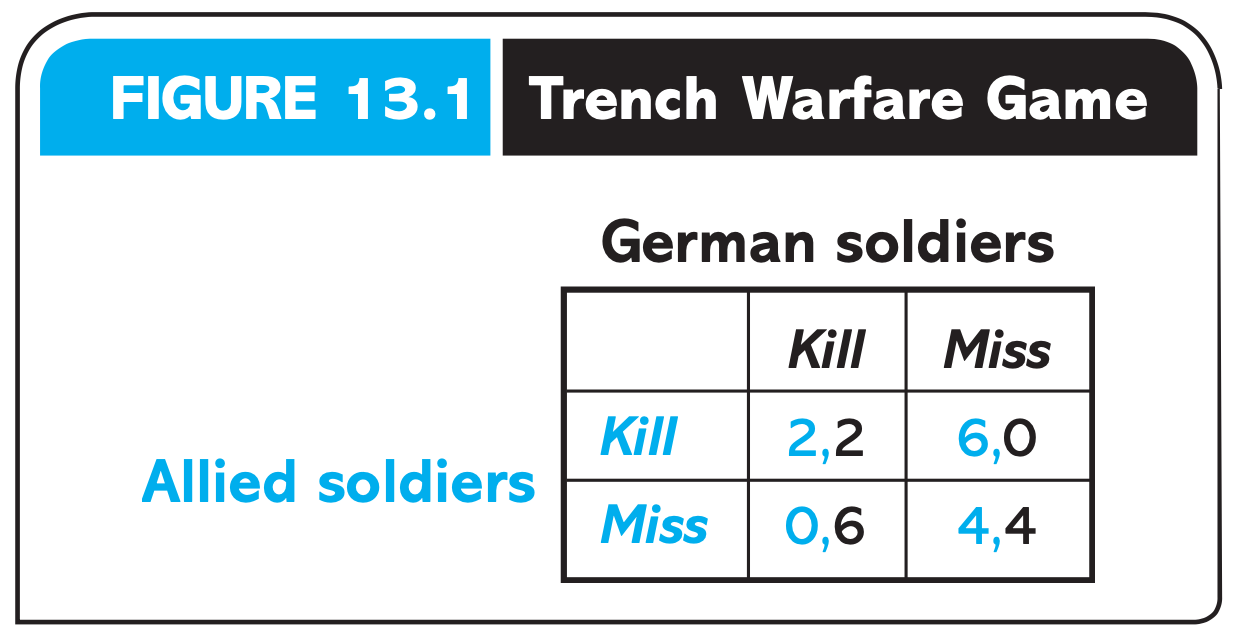
\includegraphics[width=1\textwidth]{figures/fig131.png}
  \end{center}
  What's the \textbf{NE}?
\end{frame}

\begin{frame}{Unexpected Truces Emerge}
  Christmas Day Truce, 1914:
  \begin{center}
    \includegraphics[width=.75\textwidth]{figures/hughes24-superJumbo.png} 
  \end{center}
  {\footnotesize Image Credit: Stephanie Lecocq/European Pressphoto Agency}
\end{frame}

\begin{frame}{Unexpected Truces Emerge}
  \begin{quote}
    \footnotesize 

    So regular were [the Germans] in their choice of targets, times of shooting, and number of rounds fired, that, after being in the line one or two days, Colonel Jones had discovered their system, and knew to a minute where the next shell would fall. His calculations were very accurate, and he was able to take what seemed to uninitiated Staff Officers big risks, knowing that the shelling would stop before he reached the place being shelled.

    I was having tea with A Company when we heard a lot of shouting and went out to investigate. We found our men and the Germans standing on their respective parapets. Suddenly a salvo arrived but did no damage. Naturally both sides got down and our men started swearing at the Germans, when all at once a brave German got on to his parapet and shouted out “We are very sorry about that; we hope no one was hurt. It is not our fault, it is that damned Prussian artillery.”
  \end{quote} 
\end{frame}

\begin{frame}{The puzzle of trench truces}
  \begin{itemize}
    \item How did cooperation between enemy armies achieved and sustained?
    \item One answer might be that in these parts of the front, interactions were \textbf{repeated} between the same units
  \end{itemize} 
\end{frame}

\begin{frame}{Constructing a Repeated Game}
  \begin{itemize}
    \item Suppose that Allied and German forces anticipate that they will play this game $T$ times 
  \end{itemize}
  \begin{center}
    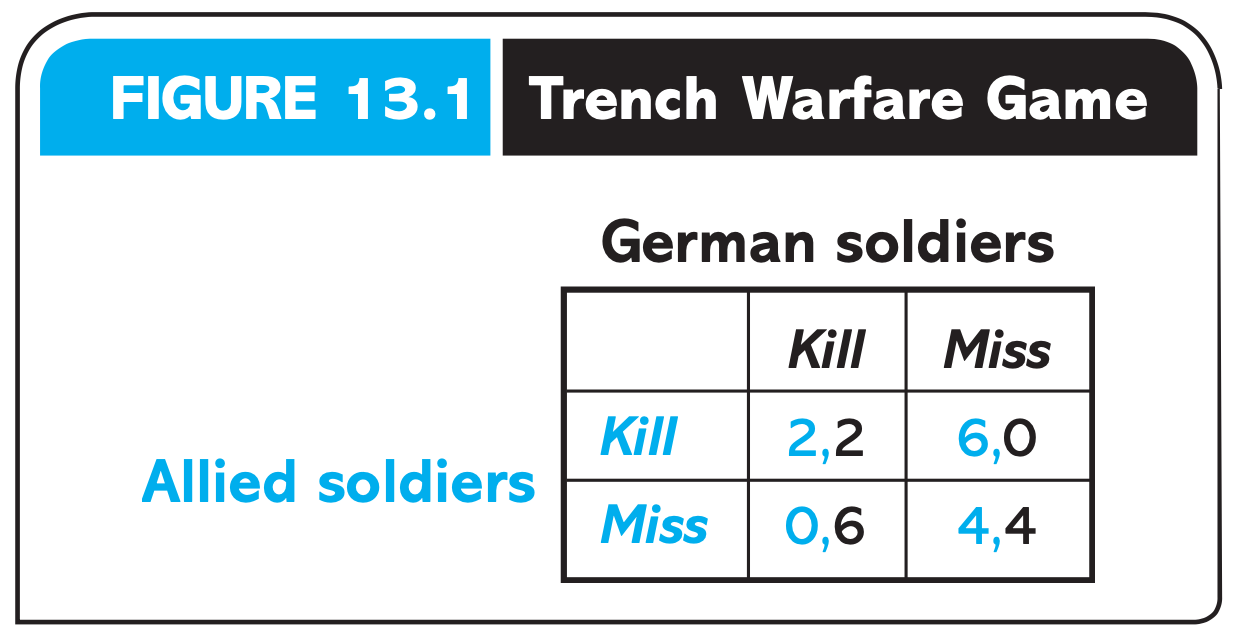
\includegraphics[width=.5\textwidth]{figures/fig131.png}  
  \end{center}
  \begin{itemize}
    \item A \textit{strategy} will be made up of $T$ \textit{actions}; 
    one for each time this stage game is played
  \end{itemize}
\end{frame}

% \begin{frame}{Constructing a Repeated Game}
%   To represent this as an extensive form tree, lets suppose that $T=2$:
%   \begin{itemize}
%     \item If neither side sees what their opponent's strategy was yesterday, each player has 3 info sets
%     \item So each side has eight possible strategies:
%     \begin{itemize}
%       \item (\textit{Kill$_1$}, \textit{Kill$_2$} if \textit{Kill$_1$} or \textit{Miss$_1$})
%       \item (\textit{Kill$_1$}, \textit{Kill$_2$} if \textit{Kill$_1$} else \textit{Miss$_2$} if \textit{Miss$_1$})
%       \item (\textit{Kill$_1$}, \textit{Miss$_2$} if \textit{Kill$_1$} else \textit{Kill$_2$} if \textit{Miss$_1$})
%       \item (\textit{Kill$_1$}, \textit{Miss$_2$} if \textit{Kill$_1$} or \textit{Miss$_1$})
%       \item ...
%     \end{itemize}
%   \end{itemize}
% \end{frame}

% \begin{frame}{Constructing a Repeated Game}
%   \begin{center}
%     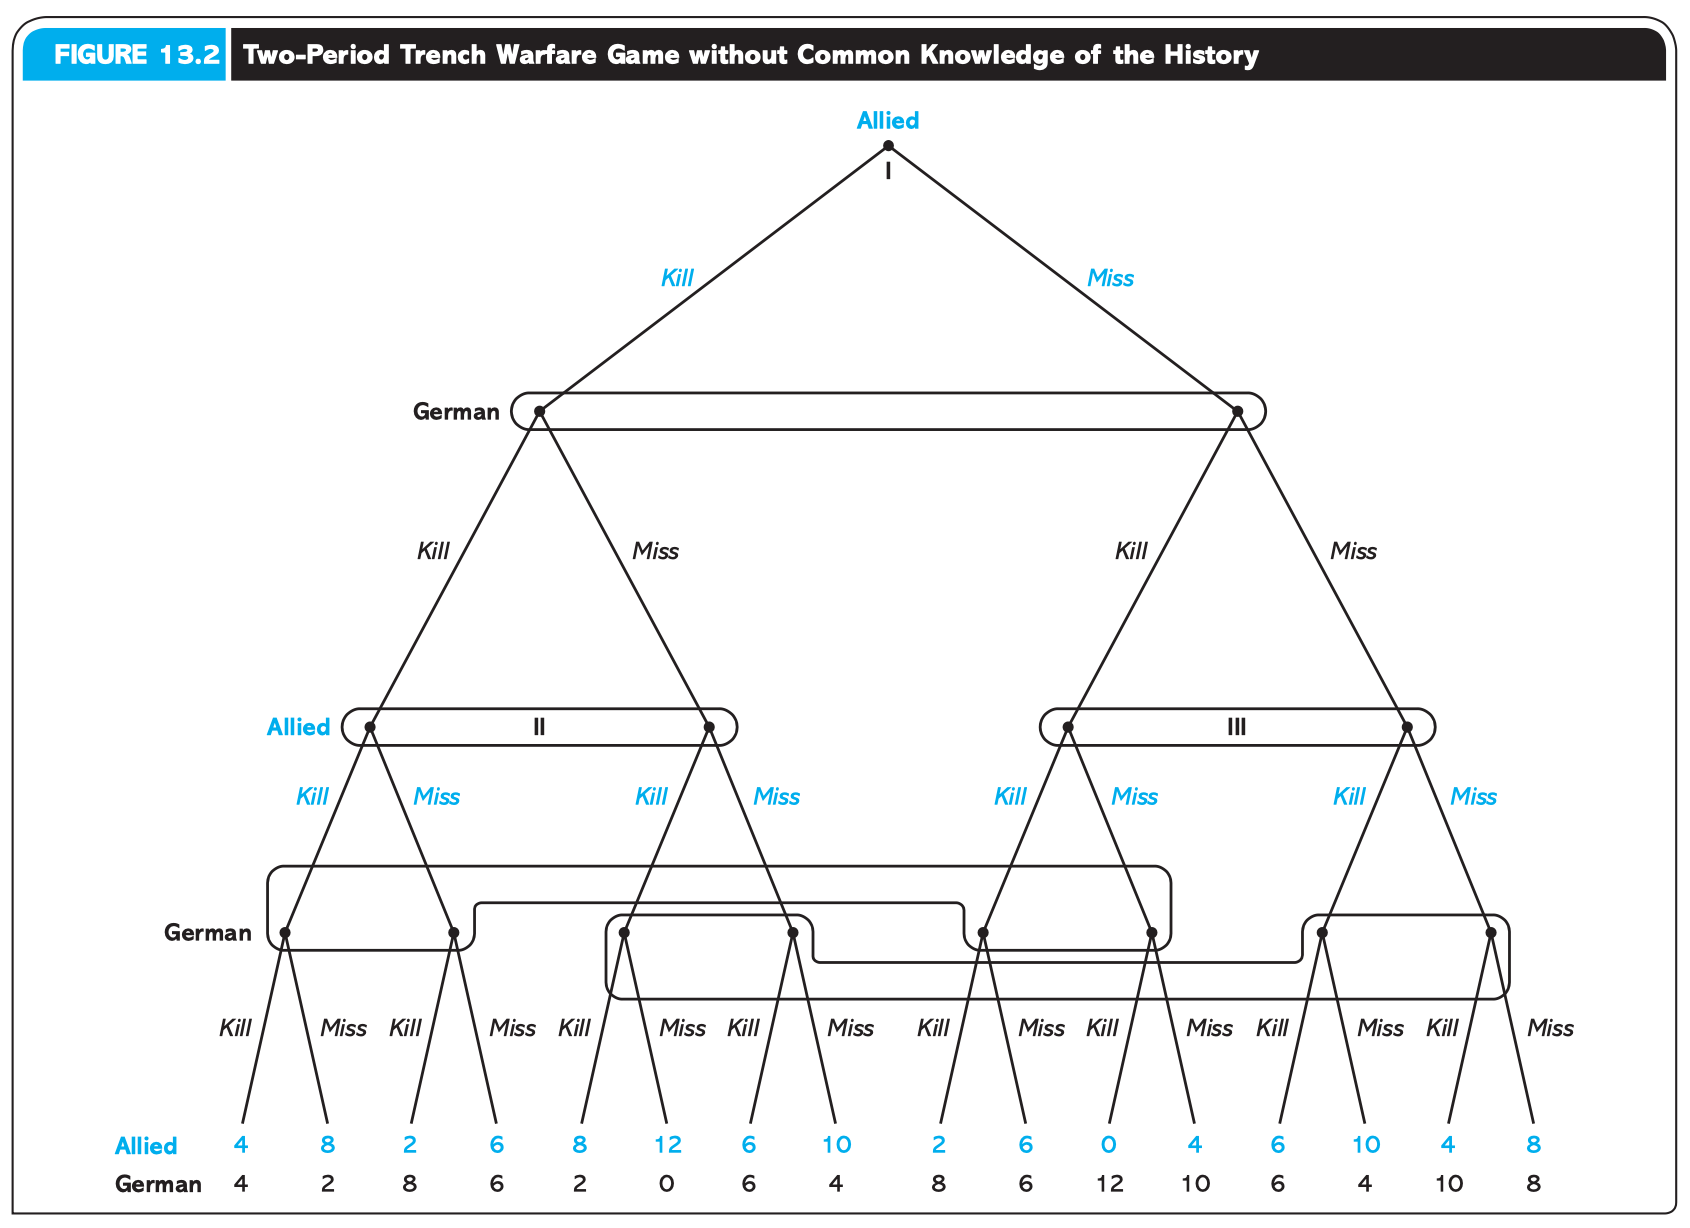
\includegraphics[width=1\textwidth]{figures/fig132.png} 
%   \end{center} 
% \end{frame}

\begin{frame}{Constructing a Repeated Game}
  To represent this as an extensive form tree, lets suppose that $T=2$:
  and suppose that the history of all past plays are \textbf{common knowledge} 
  \begin{itemize}
    \item each player will have five info sets; one for day 1, and four in day 2 
    \item What does the extensive form game look like?
  \end{itemize}
\end{frame}

\begin{frame}{Constructing a Repeated Game}
  \begin{center}
    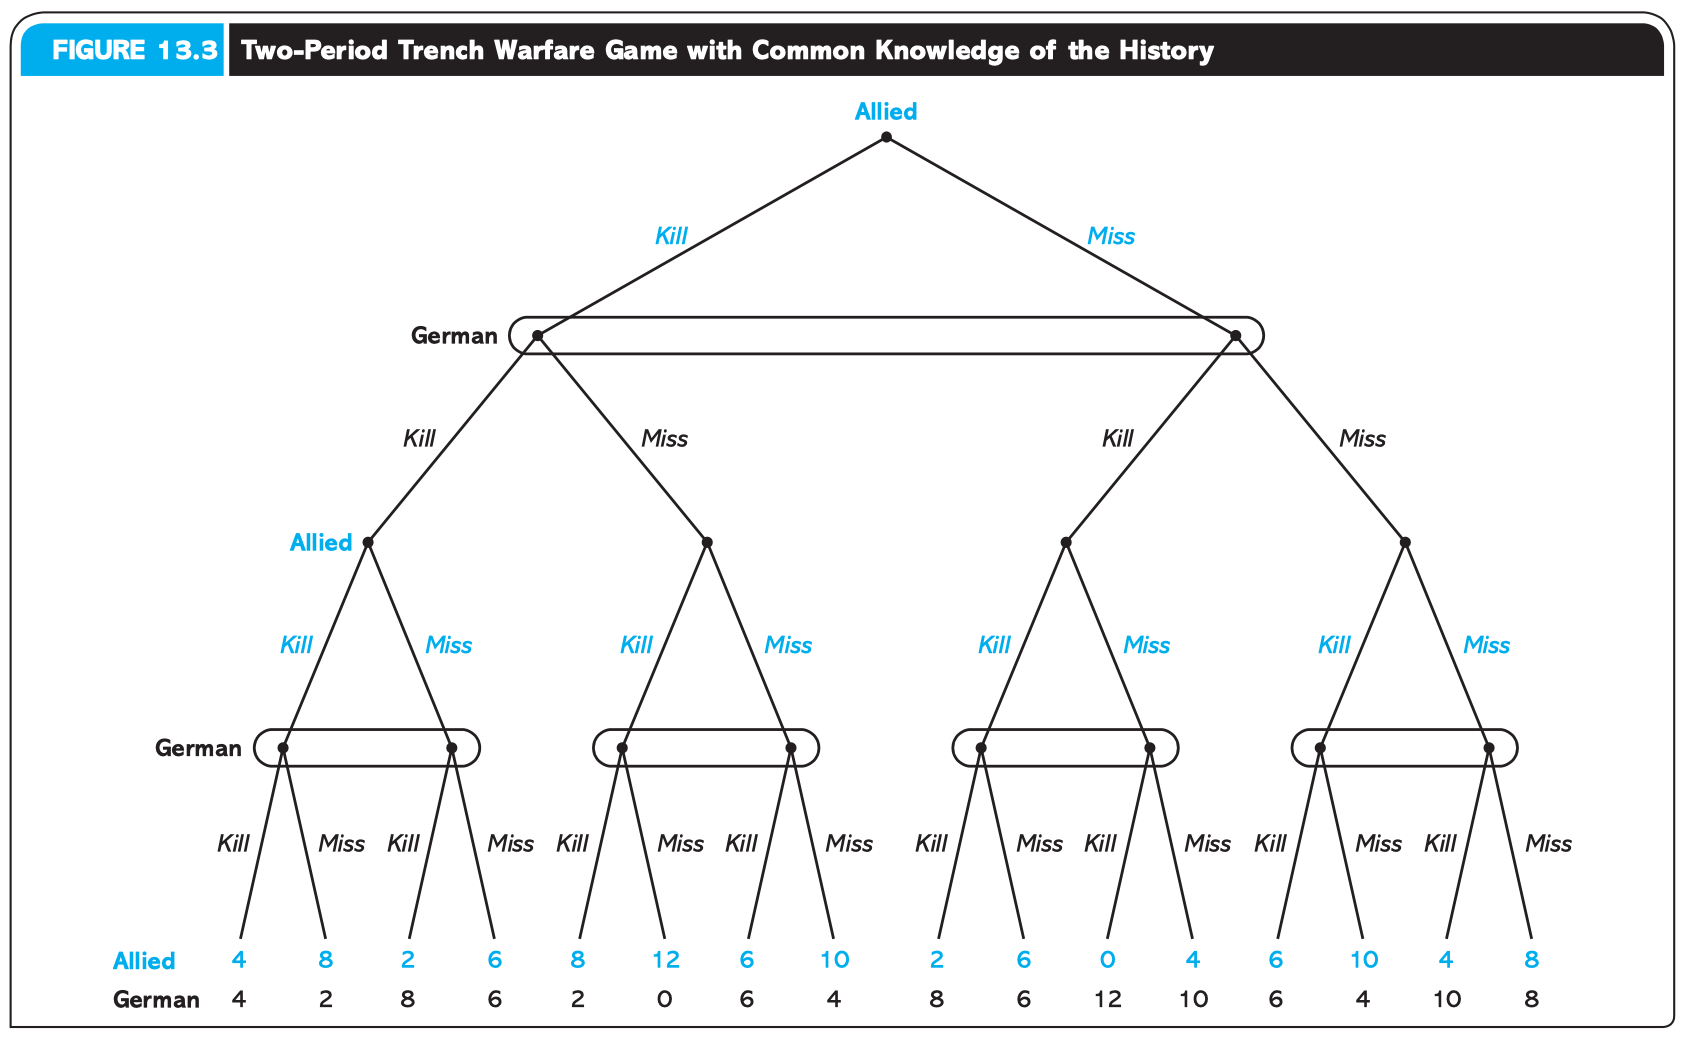
\includegraphics[width=1\textwidth]{figures/fig133.png} 
  \end{center} 
\end{frame}

\begin{frame}{Constructing a Repeated Game}
  Let's generalize what a strategy in \textit{any} \alert{finitely repeated game} with \alert{common knowledge} will look like:
  \begin{itemize}
    \item If a game has $T$ periods, and each player has $m$ actions at each stage,
    \item there is one initial info set, $m^2$ info sets in period 2, $m^4$ info sets in period 3, ..., $m^{2(T-1)}$ in the last period 
    \item A complete strategy is made up of $1 + m^2 + m^4 + ... + m^{2(T-1)}$ actions 
  \end{itemize}
  In an \alert{infinitely repeated game}, there will be an infinite number of actions in each strategy
\end{frame}

\begin{frame}{Constructing a Repeated Game}
  How to model streams payoffs over time?
  \begin{itemize}
    \item We could just add up all of the per-stage payoffs across an entire history
    \item But for infinitely-long histories, this sum would blow up and not make much sense
    \item Instead, we will use \alert{present value} calculations
  \end{itemize}
\end{frame}

\begin{frame}{Present Values}
  Suppose that I have an income stream where I earn $w_t$ dollars in every year $t$
  \begin{itemize}
    \item Suppose that there is a single \alert{discount factor} $\delta$ which captures how much I value income tomorrow compared to income today
    \item My present value over my whole income stream is 
    $$ w_1 + \delta w_2 + \delta^2 w_3 + \delta^3 w_4 + ... + \delta^{T-1} w_T $$
    \item It makes sense to assume that $0<\delta<1$ because I should probably care about tomorrow to some extent, but not as much as today
  \end{itemize}
\end{frame}

\begin{frame}{Present Values}
  What about calculating a present value of an \alert{infinte stream} of payoffs?
  \begin{itemize}
    \item It turns out:  
    $$ x + \delta x + \delta^2 x + \delta^3 x + ... + \delta^{\infty} x $$
    \item actually converges to $\frac{x}{1-\delta}$ as long as $\delta<1$ 
  \end{itemize}
\end{frame}

\begin{frame}{Check Your Understanding}
  Suppose you are deciding between three different payoff streams:
  \vspace{5mm}

  \begin{center}
  \begin{tabular}{|c|c|c|c|}
    \textbf{Period} & \textbf{Stream A} & \textbf{Stream B} & \textbf{Stream C} \\ \hline 
    1 & 15 & 25 &  5 \\ 
    2 & 15 & 15 & 10 \\ 
    3 & 15 & 10 & 20 \\ 
    4 & 15 &  5 & 30 \\
  \end{tabular}
  \end{center}

  \vspace{5mm}
  Which has the \textbf{highest present value} when $\delta =0.8$?
  \pause
  
  Stream A: 44.28, \textbf{Stream B: 45.9}, Stream C: 41.16
\end{frame}

\begin{frame}{Going back to the trenches}
  \begin{center}
    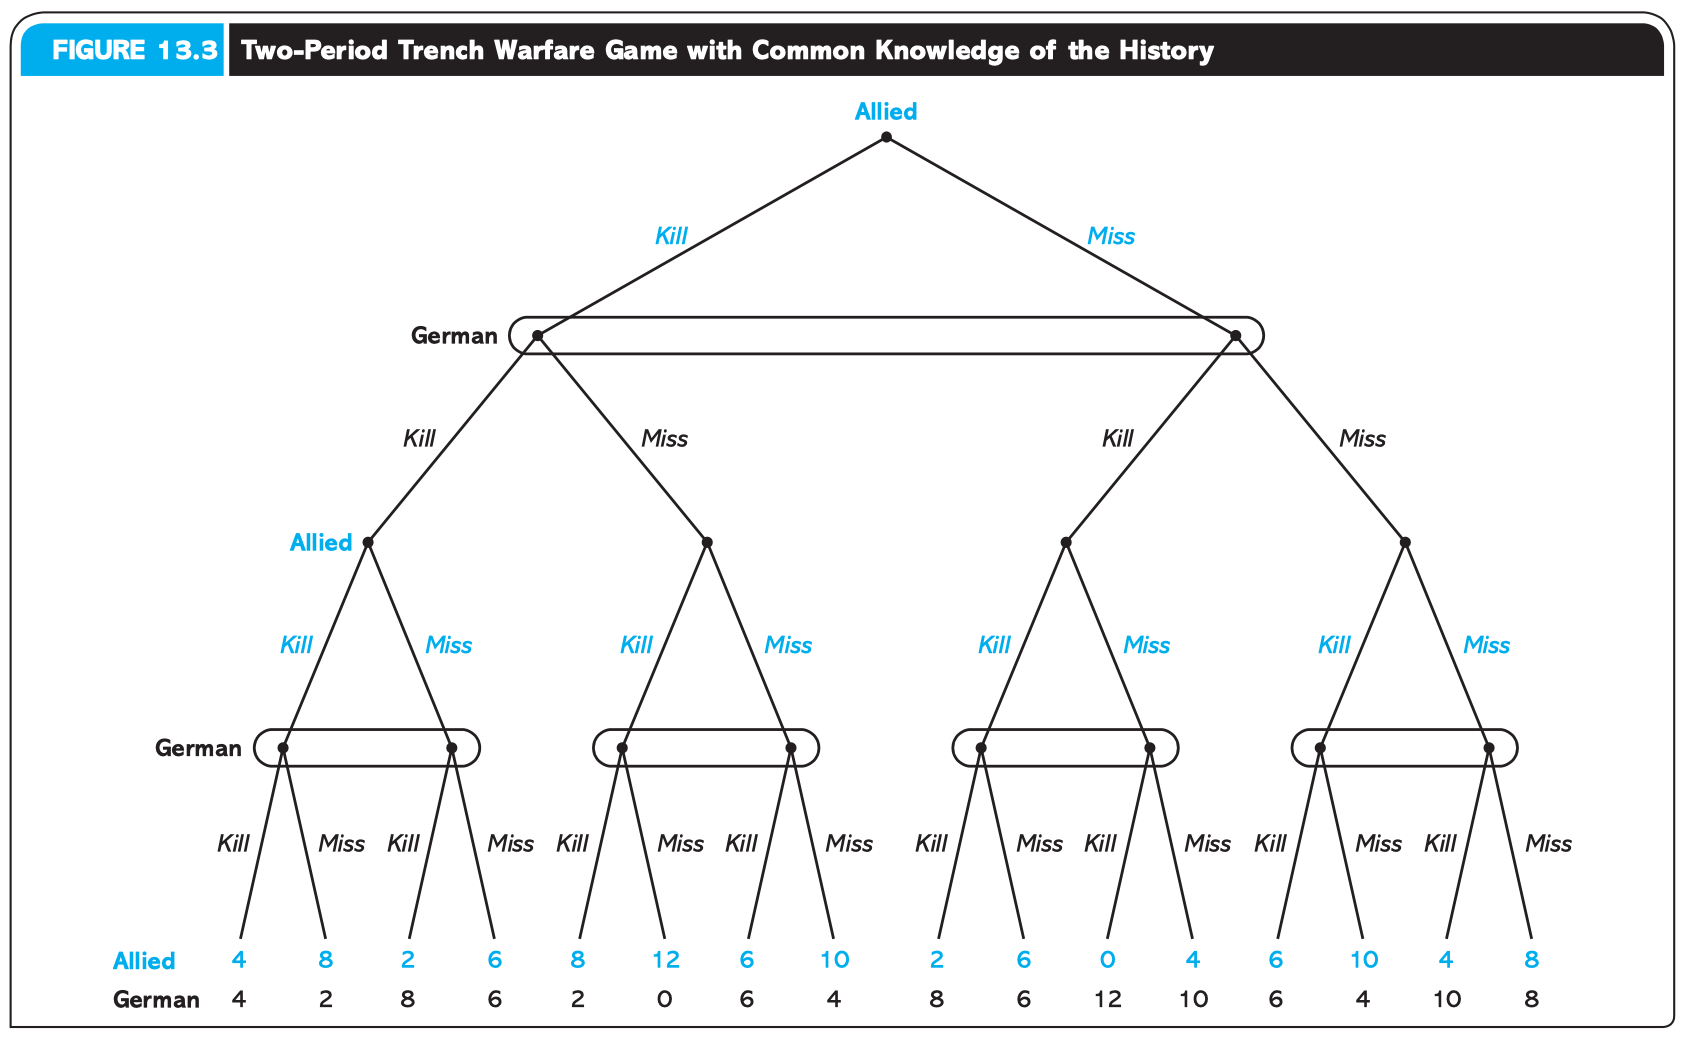
\includegraphics[width=.8\textwidth]{figures/fig133.png} 
  \end{center}  
  This was our extensive form game for only 2 periods
\end{frame}

\begin{frame}{Going back to the trenches}
  Now suppose that we have a potentially very large $T$

  How can we find a SPNE?

\end{frame}

\begin{frame}{Going back to the trenches}
  Suppose that we are already at the last period $T$ of the $T$-period trench warfare game 

  Suppose that the Allies total payoff stream value so far is $A^{T-1}$ and the Germans is $G^{T-1}$ 
  \begin{center}
    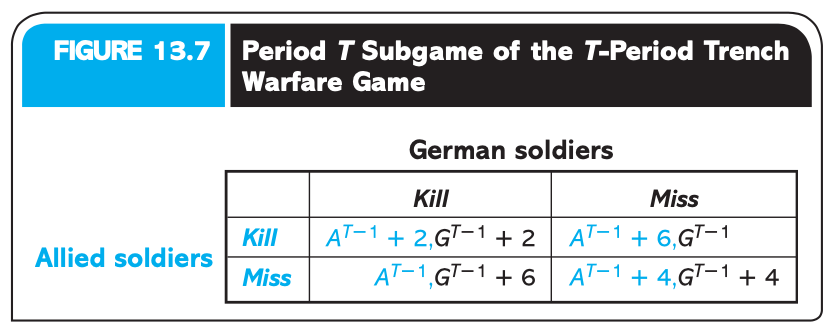
\includegraphics[width=.7\textwidth]{figures/tab137.png} 
  \end{center}
  What will happen?
  \pause

  \begin{itemize}
      \item Allies will Shoot to \textbf{Kill},
      Germans will Shoot to \textbf{Kill}
  \end{itemize}
\end{frame}

\begin{frame}{Going back to the trenches}
  Now that we know the $T$ stage will end in $(Kill, ~Kill)$, we can look one period back to what will happen in $T-1$: 
  \begin{center}
    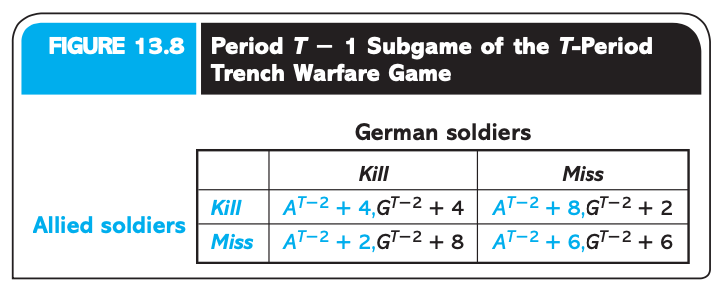
\includegraphics[width=.7\textwidth]{figures/fig138.png}
  \end{center}
  What will happen?
  \pause
  \begin{itemize}
      \item Both will shoot to \textbf{Kill} in $T-1$, knowing they will both shoot to kill in $T$
  \end{itemize}
\end{frame}

\begin{frame}{Trench Game with Finite stages}
  By now, you should get the idea:
  \begin{block}{Insight}
    If the stage game has a unique NE, then any finitely repeated version will have a unique SPNE which is just the repetition of the single-stage NE. No cooperation is sustainable 
  \end{block}

  So what was going on with those spontaneous truces?
\end{frame}

\begin{frame}{Infinitely Repeated Trench Game}
  \begin{itemize}
    \item The problem with that last equilibrium we found was that you have to know \textit{exactly when the game will end} to use backwards induction 
    \item But for World War I infantrymen, they didn't know how long it would be until the fronts shifted or their division was rotated out
    \item We will have to extend our models to allow for \alert{indefinite horizons}
  \end{itemize} 
\end{frame}

\begin{frame}{Infinitely Repeated Games}
  Suppose the probability that at each stage, with probability $p$, the game continues and with $(1-p)$, the game ends and you get $u=0$

  The \textbf{expected present value} of a stream of payoffs $u_1, u_2, ...$ is then:
  $$ V = u_1 + p d u_2 + p^2 d^2 u_3 + ... = \sum_{t=1}^{\infty}(pd)^{t-1}u_t $$
\end{frame}

\begin{frame}{Infinitely Repeated Games}
  Now if we let $\delta = pd$ represent the discount factor from both time preferences and the likelihood of the game terminating:
  $$ V = \sum_{t=1}^{\infty}(pd)^{t-1}u_t = \sum_{t=1}^{\infty}\delta^{t-1}u_t $$

  Which is exactly the same as the expected present value of a stream of \textbf{infinite} payments
\end{frame}

\begin{frame}{SPNE in Repeated Games}
  A strategy profile is SPNE if and only if in each period and for each history, the prescribed action is optimal given:
  \begin{itemize}
    \item the other players act according to their strategies in the current period
    \item all players act according to their strategies in all future periods
  \end{itemize}
\end{frame}

\begin{frame}{Grim Trigger in the Trench Game}
  Consider the following strategy: 
  \begin{itemize}
    \item In period 1, choose miss
    \item In period $t>1$, choose miss if both chose miss in all past periods, else choose kill
  \end{itemize}
  This type of strategy is known as \alert{Grim Trigger} because this type of player starts out cooperative, but if wronged once, they will always shoot to kill
\end{frame}


\section*{General Repeated Prisoners' Dilemma}
% Section 2: General-Form Prisoners' Dilemma Repeated
%-------------------------------------------------------------------------------

\begin{frame}{General Prisoners' Dilemma}
  \begin{table}[!h]
    \centering
    \begin{tabular}{*{4}{c|}}
      \multicolumn{2}{c}{} & \multicolumn{2}{c}{Column} \\ \cline{3-4}
      \multicolumn{1}{c}{} &         & Defect  & Cooperate \\ \cline{2-4}
      \multirow{2}*{Row} &    Defect & $D$,$D$ & $H$,$L$   \\ \cline{2-4}
                         & Cooperate & $L$,$H$ & $C$,$C$   \\ \cline{2-4} 
    \end{tabular} 
  \end{table} 

  What ordering of payoffs $D$, $H$, $L$, and $C$ make this a \textbf{Prisoners' Dilemma}? 
  \begin{enumerate}[label=\textbf{\alph*)}]
    \item $C > D > H > L$ 
    \item $H > D > C > L$ 
    \item $H > C > D > L$ 
    \item $C > H > L > D$
  \end{enumerate}
  \pause 

  Answer: \textbf{(c)}!
\end{frame}

\begin{frame}{General Prisoners' Dilemma}
  A single-stage prisoners' dilemma in extensive form:
  \usetikzlibrary{calc} 
  \begin{center}
  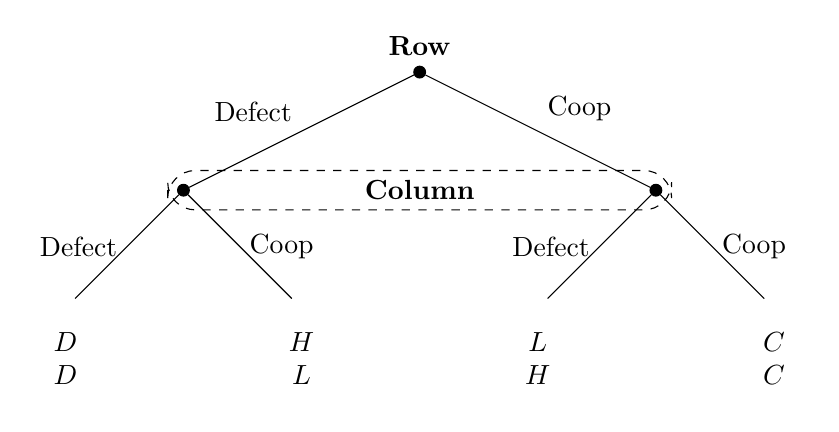
\begin{tikzpicture}
    \tikzstyle{solid node}=[circle,draw,inner sep=1.5,fill=black]
    \tikzstyle{level 1}=[level distance=15mm,sibling distance=6cm]
    \tikzstyle{level 2}=[level distance=15mm,sibling distance=3cm]
    \node(0)[solid node,label=above:{\textbf{Row}}]{}
        child{node(1)[solid node,label=above left:{}]{}
            child{node[label=below:{\begin{tabular}{c}
                    $D$ \\
                    $D$
                \end{tabular}}]{} edge from parent node[left]{Defect}}
            child{node[label=below:{\begin{tabular}{c}
                    $H$ \\
                    $L$
                \end{tabular}}]{} edge from parent node[right]{Coop}}
            edge from parent node[above left]{Defect}
        }
        child{node(2)[solid node,label=above right:{}]{}
            child{node[label=below:{\begin{tabular}{c}
                    $L$ \\
                    $H$
                \end{tabular}}]{} edge from parent node[left]{Defect}}
            child{node[label=below:{\begin{tabular}{c}
                    $C$ \\
                    $C$
                \end{tabular}}]{} edge from parent node[right]{Coop}}
            edge from parent node[above right]{Coop}
        };
    \draw[dashed,rounded corners=10]($(1) + (-.2,.25)$)rectangle($(2) +(.2,-.25)$);
    \node at($(1)!.5!(2)$){\textbf{Column}};
  \end{tikzpicture}
  \end{center}
\end{frame}

\begin{frame}{General Prisoners' Dilemma}
  A \textbf{two-stage} prisoners' dilemma in mixed extensive form:
  \usetikzlibrary{calc} 
  \begin{center}
    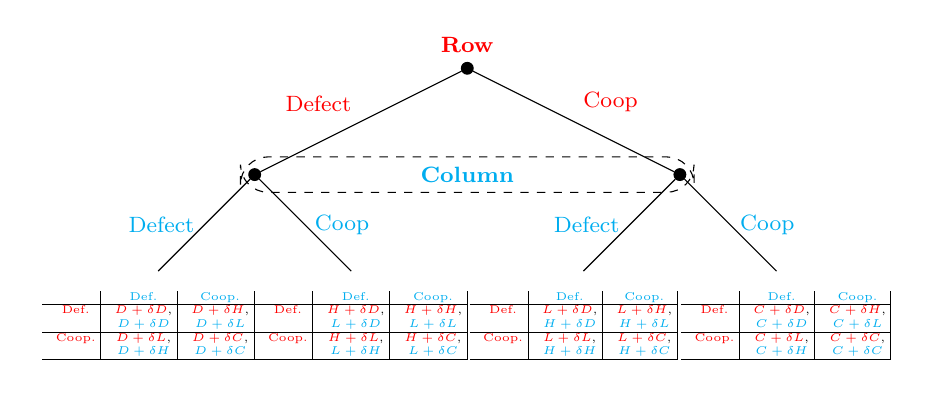
\begin{tikzpicture}[scale=0.9,font=\footnotesize]
    \tikzstyle{solid node}=[circle,draw,inner sep=1.5,fill=black]
    \tikzstyle{level 1}=[level distance=15mm,sibling distance=6cm]
    \tikzstyle{level 2}=[level distance=15mm,sibling distance=3cm]
    \node(0)[solid node,label=above:{\color{red} \textbf{Row}}]{}
      child{node(1)[solid node,label=above left:{}]{}
        child{node(3)[]{} edge from parent node[left]{\color{cyan}Defect}}
        child{node(4)[]{} edge from parent node[right]{\color{cyan}Coop}}
        edge from parent node[above left]{\color{red}Defect}
      }
      child{node(2)[solid node,label=above right:{}]{}
        child{node(5)[]{} edge from parent node[left]{\color{cyan}Defect}}
        child{node(6)[]{} edge from parent node[right]{\color{cyan}Coop}}
        edge from parent node[above right]{\color{red}Coop}
      };
    % info set
    \draw[dashed,rounded corners=10]($(1) + (-.2,.25)$)rectangle($(2) +(.2,-.25)$);
    \node at($(1)!.5!(2)$){\color{cyan} \textbf{Column}};
    % second stage
    \node[below] at(3){
      \tiny
      \scalebox{.82}{
      \begin{tabular}{*{3}{c<{\hspace{-4pt}}|}}
         & {\color{cyan} Def.} & {\color{cyan} Coop.} \\ \cline{1-3}
         {\color{red} Def.} & {\color{red} $D + \delta D$}, & {\color{red} $D + \delta H$},\\ 
                          & {\color{cyan}$D + \delta D$}  & {\color{cyan}$D + \delta L$} \\ \cline{1-3} 
         {\color{red} Coop.} & {\color{red} $D + \delta L$}, & {\color{red} $D + \delta C$},\\ 
                          & {\color{cyan}$D + \delta H$}  & {\color{cyan}$D + \delta C$} \\ \cline{1-3} 
      \end{tabular}
      }
    };
    \node[below] at(4){
      \tiny
      \scalebox{.82}{
      \begin{tabular}{*{3}{c<{\hspace{-4pt}}|}}
         & {\color{cyan} Def.} & {\color{cyan} Coop.} \\ \cline{1-3}
         {\color{red} Def.} & {\color{red} $H + \delta D$}, & {\color{red} $H + \delta H$},\\ 
                          & {\color{cyan}$L + \delta D$}  & {\color{cyan}$L + \delta L$} \\ \cline{1-3} 
         {\color{red} Coop.} & {\color{red} $H + \delta L$}, & {\color{red} $H + \delta C$},\\ 
                          & {\color{cyan}$L + \delta H$}  & {\color{cyan}$L + \delta C$} \\ \cline{1-3} 
      \end{tabular}
      }
    };
    \node[below] at(5){
      \tiny
      \scalebox{.82}{
      \begin{tabular}{*{3}{c<{\hspace{-4pt}}|}}
         & {\color{cyan} Def.} & {\color{cyan} Coop.} \\ \cline{1-3}
         {\color{red} Def.} & {\color{red} $L + \delta D$}, & {\color{red} $L + \delta H$},\\ 
                          & {\color{cyan}$H + \delta D$}  & {\color{cyan}$H + \delta L$} \\ \cline{1-3} 
         {\color{red} Coop.} & {\color{red} $L + \delta L$}, & {\color{red} $L + \delta C$},\\ 
                          & {\color{cyan}$H + \delta H$}  & {\color{cyan}$H + \delta C$} \\ \cline{1-3} 
      \end{tabular}
      }
    };
    \node[below] at(6){
      \tiny
      \scalebox{.82}{
      \begin{tabular}{*{3}{c<{\hspace{-4pt}}|}}
         & {\color{cyan} Def.} & {\color{cyan} Coop.} \\ \cline{1-3}
         {\color{red} Def.} & {\color{red} $C + \delta D$}, & {\color{red} $C + \delta H$},\\ 
                          & {\color{cyan}$C + \delta D$}  & {\color{cyan}$C + \delta L$} \\ \cline{1-3} 
         {\color{red} Coop.} & {\color{red} $C + \delta L$}, & {\color{red} $C + \delta C$},\\ 
                          & {\color{cyan}$C + \delta H$}  & {\color{cyan}$C + \delta C$} \\ \cline{1-3} 
      \end{tabular}
      }
    };
  \end{tikzpicture}
  \end{center} 
  Recall that $\delta$ is the subjective discount rate from stage to stage 
\end{frame}

% \begin{frame}{Test Your Understanding}
%   What should you do in the two-stage Prisoners' Dilemma 
%   if your opponent plays \textit{Coop} in stage 1 and \textit{Coop} in stage 2?
%   \begin{enumerate}[label=\textbf{\alph*)}]
%     \item \textit{Coop} in stage 1, \textit{Coop} in stage 2
%     \item \textit{Coop} in stage 1, \textit{Defect} in stage 2
%     \item \textit{Defect} in stage 1, \textit{Coop} in stage 2
%     \item \textit{Defect} in stage 1, \textit{Defect} in stage 2
%   \end{enumerate}
% \end{frame}

\begin{frame}{$\mathbb{T}$-stage repeated Prisoners' Dilemma}
  A complete strategy in a $\mathbb{T}$-stage repeated game will look like:
  \begin{align*}
    S_{t=1}^{\mathbb{T}} = 
    \begin{cases}
    \text{In stage } t=1 & \text{take action } A_0 \\ 
    \text{In stage } t>1 & 
    \begin{cases}
      \text{If history so far was } h_t, \text{take action } A_t(h_t) \\
      \text{Else if history was } h'_t, \text{take action } A_t(h'_t) \\ 
      ... 
    \end{cases}
    \end{cases}
  \end{align*}
  We can see that the number of possible strategies increases exponentially as $\mathbb{T}$ gets larger
\end{frame}

\begin{frame}{$\mathbb{T}$-stage repeated Prisoners' Dilemma}
  Suppose that $\mathbb{T}$ is a very large number, but we have played to the very last stage of a repeated Prisoners' Dilemma with that many stages:
  \begin{center}
    \begin{tabular}{*{4}{c|}}
      \multicolumn{2}{c}{} & \multicolumn{2}{c}{Column} \\ \cline{3-4}
      \multicolumn{1}{c}{} &        & Defect & Cooperate \\ \cline{2-4}
      \multirow{2}*{Row} & Defect   & Tot.$^R + D$, Tot.$^C + D$ & Tot.$^R + H$, Tot.$^C + L$ \\ \cline{2-4}
                         & Cooperate& Tot.$^R + L$, Tot.$^C + H$ & Tot.$^R + C$, Tot.$^C + C$ \\ \cline{2-4}
    \end{tabular} 
  \end{center}
  Let Tot.$^R$ and Tot.$^C$ represent the total payoffs that both players have earned over 
  stages 0 to $\mathbb{T} -1$
\end{frame}

\begin{frame}{$\mathbb{T}$-stage repeated Prisoners' Dilemma}
  \begin{center}
    \begin{tabular}{*{4}{c|}}
      \multicolumn{2}{c}{} & \multicolumn{2}{c}{Column} \\ \cline{3-4}
      \multicolumn{1}{c}{} &        & Defect & Cooperate \\ \cline{2-4}
      \multirow{2}*{Row} & Defect   & Tot.$^R + D$, Tot.$^C + D$ & Tot.$^R + H$, Tot.$^C + L$ \\ \cline{2-4}
                         & Cooperate& Tot.$^R + L$, Tot.$^C + H$ & Tot.$^R + C$, Tot.$^C + C$ \\ \cline{2-4}
    \end{tabular} 
  \end{center}
  Notice that the equilibrium of this subgame is still \textit{Defect}, \textit{Defect}
  because Tot.$^R$ and Tot.$^C$ are already decided by prior actions. 
\end{frame}

\begin{frame}{Repeated Prisoners' Dilemma with Uncertain Second Stage}
  Suppose that the first stage of the game is the Trenches Game:
  \begin{table}[!h]
    \centering
    \begin{tabular}{*{4}{c|}}
      \multicolumn{2}{c}{} & \multicolumn{2}{c}{German soldiers} \\ \cline{3-4}
      \multicolumn{1}{c}{} &    & Kill & Miss \\ \cline{2-4}
      \multirow{2}*{Allied Soldiers} & Kill & 4, 4 & 8, 2 \\ \cline{2-4}
                         & Miss & 2, 8 & 6, 6 \\ \cline{2-4} 
    \end{tabular} 
  \end{table}
  But with probability $p$, the game repeats in the second round 
  and with probability $1-p$, it ends after the first round
\end{frame}

\begin{frame}{Repeated Prisoners' Dilemma with Uncertain Second Stage}
  Consider the following strategy: 
  \begin{align*}
    \begin{cases}
      \text{In stage } 1 & : \textit{Miss} \\ 
      \text{In stage } 2 & : 
      \begin{cases}
        \textit{Miss} \text{  if the other player Missed in stage 1} \\ 
        \textit{Kill} \text{  if the other player Killed in stage 1}
      \end{cases}
    \end{cases}
  \end{align*}
  Let's call this strategy \textit{Punisher} because it starts off friendly, 
  but will try to punish someone who defects in the first round by defecting in the second round.
\end{frame}

\begin{frame}{Repeated Prisoners' Dilemma with Uncertain Second Stage}
  Suppose you are playing against a \textit{Punisher} in this game. 

  \begin{center}
    \begin{tabular}{*{4}{c|}}
      \multicolumn{2}{c}{} & \multicolumn{2}{c}{German soldiers} \\ \cline{3-4}
      \multicolumn{1}{c}{} &    & Kill & Miss \\ \cline{2-4}
      \multirow{2}*{Allied Soldiers} & Kill & 4, 4 & 8, 2 \\ \cline{2-4}
                         & Miss & 2, 8 & 6, 6 \\ \cline{2-4} 
    \end{tabular} 
  \end{center}

  \begin{itemize}
    \item What is your \textbf{expected utility} of playing \textit{Kill}, \textit{Kill}?
    \pause
    \item 8 in the first stage, 4 in the second stage,
    \item so $EU(Kill,~Kill) = 8 + 4p$
  \end{itemize}
\end{frame}

\begin{frame}{Repeated Prisoners' Dilemma with Uncertain Second Stage}
  Suppose you are playing against a \textit{Punisher} in this game. 

  \begin{center}
    \begin{tabular}{*{4}{c|}}
      \multicolumn{2}{c}{} & \multicolumn{2}{c}{German soldiers} \\ \cline{3-4}
      \multicolumn{1}{c}{} &    & Kill & Miss \\ \cline{2-4}
      \multirow{2}*{Allied Soldiers} & Kill & 4, 4 & 8, 2 \\ \cline{2-4}
                         & Miss & 2, 8 & 6, 6 \\ \cline{2-4} 
    \end{tabular} 
  \end{center}

  What is your \textbf{expected utility} of playing \textit{Miss, Kill}? \\
  \pause
  \begin{itemize}
      \item $4 + 8p$
  \end{itemize}
  What about from playing \textit{Kill, Miss?} \\
  \pause
  \begin{itemize}
      \item $8 + 2p$
  \end{itemize}
  Would you rather defect earlier or later?
\end{frame}

\begin{frame}{Repeated Prisoners' Dilemma with Uncertain Second Stage}
  Suppose you are playing against a \textit{Punisher} in this game. 

  \begin{center}
    \begin{tabular}{*{4}{c|}}
      \multicolumn{2}{c}{} & \multicolumn{2}{c}{German soldiers} \\ \cline{3-4}
      \multicolumn{1}{c}{} &    & Kill & Miss \\ \cline{2-4}
      \multirow{2}*{Allied Soldiers} & Kill & 4, 4 & 8, 2 \\ \cline{2-4}
                         & Miss & 2, 8 & 6, 6 \\ \cline{2-4} 
    \end{tabular} 
  \end{center}

  What is your \textbf{expected utility} of playing \textit{Miss, Miss}?
  \begin{itemize}
      \item $6 + 6p$
  \end{itemize}
\end{frame}

\begin{frame}{Repeated Prisoners' Dilemma with Uncertain Second Stage}
  Let's graph your expected utilties of each strategy:
  \begin{tikzpicture}
   \begin{axis}[
     width=0.8\textwidth,
     grid,
     xlabel={p},
     ylabel={Exp. Utility},
     xmin=0, xmax=1.0,
     ymin=4, ymax=14,
     xtick={0,.1,...,1.0},
     ytick={2, 4, 6, 8, 10, 12},
     grid style=dashed,
     legend style={tiny},
     ]
 
     \addplot[domain=0:1, samples=100, thick, red] {6 + 6*x};
     \addlegendentry{$EU(Miss, Miss)$}

     \addplot[domain=0:1, samples=100, thick, blue] {8 + 2*x};
     \addlegendentry{$EU(Kill, Miss)$}

     \addplot[domain=0:1, samples=100, thick, green] {4 + 8*x};
     \addlegendentry{$EU(Miss, Kill)$}
     
     \addplot[domain=0:1, samples=100, thick, orange] {8 + 4*x};
     \addlegendentry{$EU(Kill, Kill)$}

   \end{axis}
 \end{tikzpicture}
\end{frame}

\begin{frame}{Repeated Prisoners' Dilemma with Uncertain Second Stage}
  Now you should be getting some of the intuition for how cooperative equilibria might be achieved.
  \begin{itemize}
    \item We need the payoffs of the last period to be uncertain (or never reached)
    \item If trying to cheat a \textit{Punisher} or \textit{Grim Trigger} strategy, 
    it is better to start cheating them sooner rather than later
    \item In order for the equilibrium to have both players always cooperating,
    defecting in at least one period must not be a dominant strategy
  \end{itemize}
\end{frame}

\begin{frame}{Back to the General Form Prisoners' Dilemma}
  \begin{table}[!h]
    \centering
    \begin{tabular}{*{4}{c|}}
      \multicolumn{2}{c}{} & \multicolumn{2}{c}{Column} \\ \cline{3-4}
      \multicolumn{1}{c}{} &         & Defect  & Cooperate \\ \cline{2-4}
      \multirow{2}*{Row} &    Defect & $D$,$D$ & $H$,$L$   \\ \cline{2-4}
                         & Cooperate & $L$,$H$ & $C$,$C$   \\ \cline{2-4} 
    \end{tabular} 
  \end{table} 
  Now let's suppose that this game is repeated for an \textbf{infinite number of stages}.
\end{frame}

\begin{frame}{Extending Plays to Infinity}
  Suppose the game is in the `good' equilibrium where all players always play \textit{Cooperate}.
  \begin{itemize}
    \item What is \textbf{present value} from this equilibrium? 
    \begin{align*}
      pv\left(\{ C \}_{t=1}^{\infty}\right) & = C + \delta C + \delta^2 C + \delta^3 C + ... \\ 
         & = C \sum_{t=1}^{\infty} \delta^{t-1} \\
         & = C \frac{1}{1-\delta}
    \end{align*}
  \end{itemize}
\end{frame}

\begin{frame}{Extending Plays to Infinity}
   Let's extend the \textit{Punisher} strategy we had from the two-stage game 
   into the \textit{Grim Trigger strategy} of the general infinite horizon game:
  \begin{align*}
    \begin{cases}
      \text{In stage } 1 & : \textit{Cooperate} \\ 
      \text{In stage } t \geq 2 & : 
      \begin{cases}
        \textit{Cooperate} \text{  if only cooperation has happened so far} \\ 
        \textit{Defect} \text{  if anyone has \textit{ever} Defected in the past}
      \end{cases}
    \end{cases}
  \end{align*}
\end{frame}

\begin{frame}{Grim Trigger SPNE in Repeated PD}
  Is both players playing \textit{Grim Trigger} stable?
  \begin{itemize}
    \item Does a player have an incentive to \textit{Defect} against \textit{Grim Trigger}:
    \vspace{-5mm}
    \begin{align*}
      pv(Always~Coop) & \geq pv(Defect~once) \\
      C + \delta C + \delta^2 C + ...      & \geq H + \delta D + \delta^2 D + ...\\
      C + C \sum_{t=2}^{\infty} \delta^{t} & \geq H + D \sum_{t=2}^{\infty} \delta^{t} \\ 
      C + C \delta \sum_{t=2}^{\infty} \delta^{t-1} & \geq H + D \delta \sum_{t=2}^{\infty} \delta^{t-1} \\ 
      C + \frac{\delta C}{1 - \delta} & \geq H + \frac{\delta D}{1 - \delta} \\
      \delta & \geq \frac{H - C}{H - D}
    \end{align*}
  \end{itemize}
\end{frame}

\begin{frame}{Grim Trigger SPNE in Repeated PD}
  How do we interpret this statement:
  $$\text{Cooperation is stable when } \delta \geq \frac{H - C}{H - D}  $$ 
  \begin{itemize}
    \item Recall that the definition of the Prisoners' Dilemma was that $H > C > D > L$
    \item So this means $\frac{H - C}{H - D}$ is positive and less than 1 
    \item As the $H - C$, the relative benefit of defecting increases,
    it gets harder to sustain cooperation
    \item It also gets harder to sustain cooperation as the relative penalty of defecting, $H - D$, shrinks 
  \end{itemize}
\end{frame}

\begin{frame}{Other Strategies in Repeated Games}
  So far we've only looked at one example of a type of strategy in repeated game, 
  \textit{Grim Trigger}. 
  \begin{itemize}
    \item \underline{Can you think of some others?}
    \begin{itemize}
      \item Recall that a complete strategy for a repeated game needs: 
      \begin{itemize}
        \item An initial move at $t=1$
        \item A plan of action for \textit{every} possible history in \textit{every} later stage $t\geq2$
      \end{itemize}
      \item Ideally you would be able to tell a computer how to implement your strategy
    \end{itemize}
  \end{itemize}
\end{frame}

\begin{frame}{Other Strategies in Repeated Games}
  Telling a computer how to implement strategies is exactly what Robert Axelrod did in a famous tournament in 1980.
  \begin{itemize}
    \item He invited people to submit their programs which would play 200 rounds of the prisoners' dilemma against each other 
    \item The winning program was the one which had the highest total score after playing 200 rounds against all other programs
    \item What types of strategies do you think would succeed?
  \end{itemize}
\end{frame}

\begin{frame}{An Unexpected Winner}
  The winning program was named \texttt{TIT FOR TAT} \\ 
  Surprisingly, it was fairly simple:
  \begin{align*}
    \begin{cases}
      \text{In stage } 1 & : \textit{Cooperate} \\ 
      \text{In stage } t \geq 2 & : 
      \begin{cases}
        \text{repeat what the other player did in } t-1 \\
      \end{cases}
    \end{cases}
  \end{align*}
\end{frame}

\begin{frame}{Tit-for-Tat}
  Like \textit{Grim Trigger}, \textit{Tit-for-Tat} can punish other players for defecting. 
  \begin{itemize}
    \item If a player plays \textit{Defect}, it will copy them with \textit{Defect} next round 
  \end{itemize}
  But unlike \textit{Grim Trigger} it has a short memory; or is very forgiving
  \begin{itemize}
    \item If the player who defected goes back to playing cooperatively, 
    \textit{Tit-for-Tat} will go back to cooperating too
  \end{itemize}
\end{frame}

\begin{frame}{Axelrod's Tournament}
  If you want to learn more: 
  \begin{itemize}
    \item Read the original paper: 

    {
    \footnotesize
    Axelrod, Robert; Hamilton, William D. (27 March 1981), "The Evolution of Cooperation" (PDF), \textit{Science}, 211 (4489): 1390–96
    }

    \item The 1984 Book \textit{The Evolution of Cooperation}, Basic Books

    \item Run the tournament yourself in python!
    \url{https://github.com/Axelrod-Python/Axelrod}
    
    \item Play this fun and short web game! 
    \url{https://ncase.me/trust/}

  \end{itemize}
\end{frame}


\section*{Other Repeated Games}
% Section 3: Other Repeated Games
%-------------------------------------------------------------------------------

\begin{frame}{A More Complicated Game}
  \begin{center}
  \begin{tabular}{cr|c|c|c|}
  	& \multicolumn{1}{c}{} & \multicolumn{3}{c}{Player 2}\\ \cline{3-5}
    \multicolumn{1}{c}{} & \multicolumn{1}{c}{} & x & y & z \\\cline{2-5}
    \multirow{3}*{Player 1}  & x & 5, 5 & 2, 7 & 1, 3 \\\cline{2-5}
                             & y & 7, 2 & 3, 3 & 0, 1 \\\cline{2-5}
                             & z & 3, 1 & 1, 0 & 2, 2 \\\cline{2-5}
  \end{tabular}
  \end{center}

  What are the \textbf{pure strategy Nash equilibria} of the \textit{one-shot} game?
\end{frame}

\begin{frame}{Repeated Game with 3 strategies per period}
  Now suppose that this game is played repeatedly an infinite number of times.  
  \begin{itemize}
    \item Can we do better than the single period equilibrium? 
  \end{itemize}
\end{frame}

\begin{frame}{Grim Trigger}
  \underline{Player 1} 
  \begin{align*}
    \begin{cases}
      t = 0 & \text{Play } x  \\ 
      t > 0 & 
      \begin{cases}
        \text{Play } x \text{ if only } x \text{ has been played } \\
        \text{Play } y \text{ if anything other than } x \text{has been played} \\
      \end{cases}
    \end{cases} 
  \end{align*}

  \underline{Player 2}
  \begin{itemize}
    \item $EV_{Coop} = \frac{5}{1-\delta}$ 
    \item $EV_{Cheat} = 7 + \frac{3\delta}{1-\delta}$
  \end{itemize}
\end{frame}

\begin{frame}{Grim Trigger}
  Solve for the value of $\delta$ for which this is a \textbf{SPNE}
  \vspace{50mm}
\end{frame}

\begin{frame}{Tit-for-Tat with extra forgiveness}
  \underline{Player 1} 
  \begin{align*}
    \begin{cases}
      t = 0 & \text{Play } x  \\ 
      t > 0 & \text{Play Player 2's strategy from } t-1 \\
       & 
      \begin{cases}
        \text{If P2 didn't play } x \text{ in } t-2 \text{ and P2 did play } x \text{ in } t-1, \\ 
        \text{ play P2's strategy from } t-1 \\ 
        \text{Else play } y \text{ forever} \\
      \end{cases}
    \end{cases} 
  \end{align*}

  \underline{Player 2}
  \begin{itemize}
    \item $EV_{Coop} = \frac{5}{1-\delta}$ 
    \item $EV_{Cheat} = 7 + 2\delta + \frac{5\delta^2}{1-\delta}$
  \end{itemize}
\end{frame}

\begin{frame}{Tit-for-Tat with extra forgiveness}
  Solve for the value of $\delta$ for which this is a \textbf{SPNE}
  \vspace{50mm}
\end{frame}

\begin{frame}{Tit-for-Tat vs Grim Trigger}
  Tit-for-Tat is more forgiving
  \begin{itemize}
    \item If $\delta \geq 1/2$, equilibrium is supported by Grim Trigger 
    \item If $\delta \geq 2/3$, equilibrium is supported by Tit-for-Tat
  \end{itemize}
\end{frame}

\begin{frame}{A reciprocating cooperation strategy}
    \underline{Player 1}
    $
      \begin{cases}
        t=0 & \text{Play } y \\ 
        t>0 & 
        \begin{cases}
          \text{Play } y \text{ if } t \text { is even } \\ 
          \text{Play } x \text{ if } t \text { is odd } \\ 
          \text{Play } z \text{ forever } \\
          \text{ if P2 played } y \\ 
          \text{ when $t$ is even} \\ 
        \end{cases}
      \end{cases} 
    $

    \underline{Player 2}
    $
      \begin{cases}
        t=0 & \text{Play } x \\ 
        t>0 & 
        \begin{cases}
          \text{Play } y \text{ if } t \text { is odd } \\ 
          \text{Play } x \text{ if } t \text { is even } \\ 
          \text{Play } z \text{ forever } \\
          \text{ if P2 played } y \\ 
          \text{ when $t$ is odd} \\ 
        \end{cases}
      \end{cases} 
      $
\end{frame}

\begin{frame}{A reciprocating cooperation strategy}
  Solve for the value of $\delta$ for which this is a \textbf{SPNE}
  \vspace{50mm}
\end{frame}

\begin{frame}{When can cooperation be achieved?}
  With all of these different ways of achieving repeated cooperation, 
  you might be wondering if there is a way to tell what strategies can actually work
\end{frame}

\begin{frame}{Folk Theorem}
  Any strategy is a potential SPNE for a \textbf{repeated} stage game if: 
  \begin{itemize}
    \item Both agents are sufficiently patient and far-sighted (high enough $\delta$)
    \item The payoffs from the cooperative strategy profile satisfy the two properties: 
    \begin{itemize}
      \item \textbf{Individually Rational:} the payoffs to each agent (weakly) exceed their minimax payoffs in the stage game 
      \item \textbf{Feasibility:} the payoffs are weighted averages of the payoffs found in the stage game
    \end{itemize}
  \end{itemize}
\end{frame}

\begin{frame}{Folk Theorem with 3x3 Repeated Game Example}
  \begin{center}
  \begin{tabular}{cr|c|c|c|}
  	& \multicolumn{1}{c}{} & \multicolumn{3}{c}{Player 2}\\ \cline{3-5}
    \multicolumn{1}{c}{} & \multicolumn{1}{c}{} & x & y & z \\\cline{2-5}
    \multirow{3}*{Player 1}  & x & 5, 5 & 2, 7 & 1, 3 \\\cline{2-5}
                             & y & 7, 2 & 3, 3 & 0, 1 \\\cline{2-5}
                             & z & 3, 1 & 1, 0 & 2, 2 \\\cline{2-5}
  \end{tabular}
  \end{center}

  The \alert{Minimax} equilibrium is (z,z)
  \begin{itemize}
    \item it \textit{minimizes} the \textit{maximum} payoff that your opponent could get
    \item The Minimax payoffs in this stage game are (2, 2)
    \item Intuitively, this is the \textit{safe} option: you can always fall back on it if cooperation fails
  \end{itemize}
\end{frame}

\begin{frame}{Folk Theorem with 3x3 Repeated Game Example payoffs}
  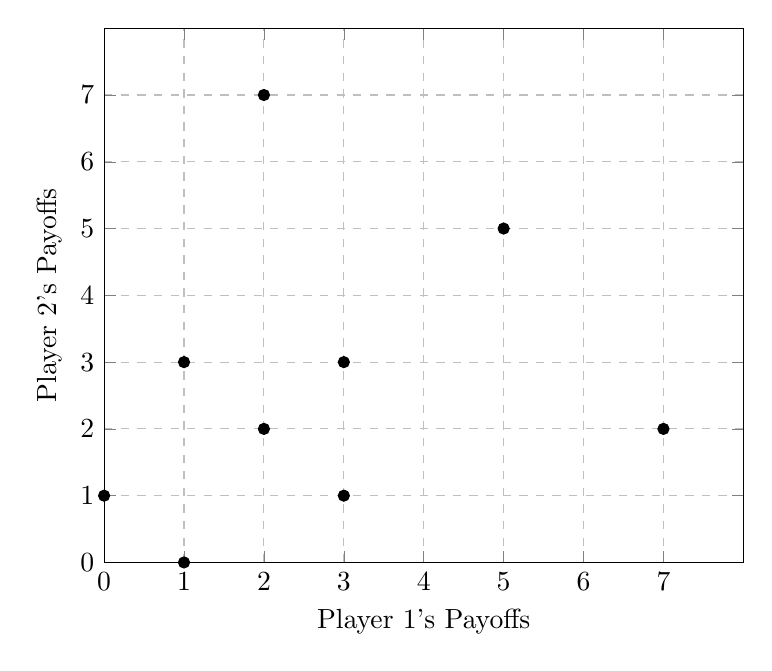
\begin{tikzpicture}
   \begin{axis}[
     width=0.8\textwidth,
     grid,
     xlabel={Player 1's Payoffs},
     ylabel={Player 2's Payoffs},
     xmin=0, xmax=8,
     ymin=0, ymax=8,
     xtick={0,1,...,7},
     ytick={0,1,...,7},
     grid style=dashed,
     ]
 
     \addplot[only marks]
     coordinates {
     (5,5) (2,7) (1,3) 
     (7,2) (3,3) (0,1)
     (3,1) (1,0) (2,2)
     };
   \end{axis}
 \end{tikzpicture}
\end{frame}

\begin{frame}{Folk Theorem with 3x3 Repeated Game Example}
  \begin{itemize}
    \item The shaded region of the graph shows us all of the strategy profiles which could be sustained by the \textbf{Folk Theorem} 
    \item This shows us why that strategy profile of alternating between (x, y) and (y, x) worked: 
    \begin{itemize}
      \item even though getting 2 on even or odd periods was no better than the Minimax payoffs, because you could alternate with the higher payoff of 7 you could do better as long as you are patient enough 
      \item this mix between (2, 7) and (7, 2) is \textit{within the convex hull} of sustainable payoffs
    \end{itemize}
  \end{itemize} 
\end{frame}

\begin{frame}{Cooperation in Repeated Games}
  \begin{itemize}
    \item As you can probably tell, there are an infinite number of strategy profiles which can achieve cooperation 
    \begin{itemize}
      \item We could allow for mixed strategies, which would work similar to the alternating example we saw 
      \item The Folk Theorem tells us that all we need is for all players to be patient enough 
      \item and also that the past plays are common knowledge
    \end{itemize}
  \end{itemize}
\end{frame}

\begin{frame}{Importance of the Folk Theorem}
  Why does this matter for real life? 
  \begin{itemize}
    \item Most strategic interactions in your life are repeated 
    \begin{itemize}
      \item Sharing chores with your roommates 
      \item Interacting in class with me every week
      \item Being nice to the barista at your regular cafe
    \end{itemize}
  \end{itemize}
\end{frame}

\begin{frame}{Importance of the Folk Theorem}
  \begin{itemize}
    \item Even when you don't repeatedly interact with the same exact people, you still see cooperative outcomes 
    \item \textbf{Institutions, Reputations, and Social Structures} all serve to allow for past interactions to be common knowledge
    \item The history of humanity is built on how we arrange our strategic interactions in ways so that people are incentivized to play nice with others
  \end{itemize}
\end{frame}

\begin{frame}{Importance of the Folk Theorem}
  Some caveats:
  \begin{itemize}
    \item People can't know exactly when the game will end; if they don't have any incentive from future cooperative gains, they will always defect
    \begin{itemize}
      \item Institutions have to \textit{seem} like they are infinitely lived (compared to finitely lived humans)
    \end{itemize}
    \item Cooperative equilibria must be better than peoples' outside options 
    \begin{itemize}
      \item If you make your institution too costly for people to engage with, they will opt out 
    \end{itemize}
    \item People need to be patient enough to make cooperation worth it
  \end{itemize}
\end{frame}


\end{document}
